\cleardoublepage

\chapter{Comando y control}
\label{makereference6}

Teniendo disponible toda la información necesaria para el control de vuelta al \gls{bess}, es necesario convertirla a la señales que la batería entienda. A su vez, también se necesita comunicar las ofertas de compra y venta de energía al mercado, para garantizar la sincronía de las operaciones entre la carga y compra y descarga y venta de la energía, respectivamente.

Más allá de las operaciones mismas, en entornos industriales donde se mueven grandes cantidades de energía, como el pertinente, es altamente recomendable disponer de algún tipo de método con el que comprobar la correcta operación del sistema y modificar su comportamiento si resulta oportuno. Por ello, también se desarrolla un cuadro de mando con el que realizar las tareas de supervisión.

De esta forma, el apartado~\ref{makereference6.1} describe la operación automática del control de las consignas de la batería y las ofertas de mercado, mientras que el apartado~\ref{makereference6.2} detalla la implementación del cuadro de mando con el que supervisar la operación del sistema.

\section{Consignación operativa}
\label{makereference6.1}

La consignación operativa no solo incluye la señalización del perfil de carga y descarga de las baterías y es que, si el sistema no comunica adecuadamente sus intenciones de compra y venta mediante los medios preestablecidos, la entidad energética dueña de la instalación podría incurrir severas multas por incumplir el reglamento.

Con ello, el sistema debe responder a las preguntas acerca de cuándo y cuánta energía ciclar físicamente y a qué precio.

\subsection{Señalización de baterías}
\label{makereference6.1.1}

Las señales de los \gls{bess} se comunican en términos de energía, como se describe en la sección~\ref{makereference3.2}. Esto significa que a las baterías no se les pueden mandar consignas de cargar o descargar una cantidad determinada de energía por cada periodo de mercado, aunque este sea el formato de salida de la optimización. Precisamente, la razón de esta limitación es bastante sencilla: la energía es dependiente del tiempo. La potencia, en cambio, es instantánea.

Resulta que, al igual que todo el resto de activos energéticos, la operación de los \gls{bess} se mide en términos de potencia, representando el ritmo con el cual la batería transfiere energía.

Dependiendo de la posición de arbitraje, la batería puede encontrarse en diferentes perfiles de potencia, desde la inactividad y el llamado mínimo técnico, hasta el máximo operacional. En la figura~\ref{fig:perfil-potencia} se puede observar la modulación del perfil de potencia de la batería.

\begin{figure}
  \centering
  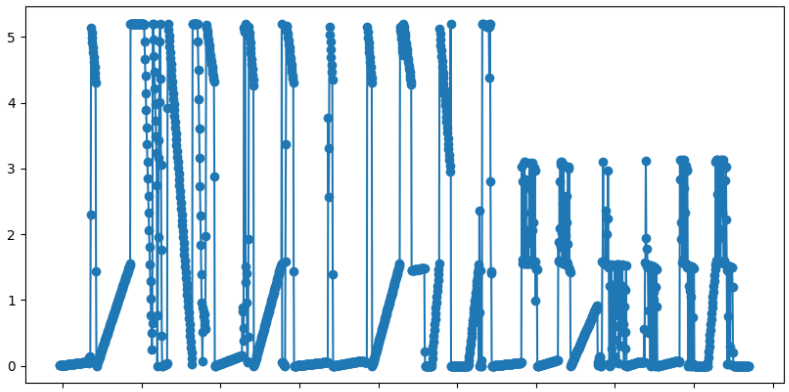
\includegraphics[width=0.75\linewidth]{figures/perfil-potencia.png}
  \caption[Modulación del perfil de potencia de una batería.]{Modulación del perfil de potencia de carga una batería de \SI{5}{\mega\watt}, en donde la potencia de carga fluctúa entre el mínimo técnico y máximo operacional, hasta verse finalmente limitada a poco más de la mitad de la potencia nominal.}
  \label{fig:perfil-potencia}
\end{figure}

Con esto, las mayores ventajas de las baterías son su capacidad de rápida conmutación o variación de su perfil de potencia y el mínimo de técnico nulo, con el que la batería puede mantenerse inactiva sin perder capacidad de conmutación.

Para transformar la posición de mercado de energía a potencia es necesario conocer el periodo o granularidad del mercado y realizar la transformación a través de la simple ecuación~\ref{eq:energia-a-potencia}. Las limitaciones de potencia ya se han tenido en cuenta en las etapas anteriores.

\begin{samepage}

  \begin{equation}
    \label{eq:energia-a-potencia}
    P_{t} = E_{t} \cdot \frac{1}{\Delta t \cdot \frac{\SI{1}{\hour}}{\SI{60}{\minute}}}
  \end{equation}

  donde

  \begin{itemize}

    \item \( P_{t} \) es la potencia a mantener durante el periodo \( t \) para ciclar una cantidad de energía en \si{\mega\watt}.

    \item \( E_{t} \) es la energía a ciclar en el periodo \( t \) en \si{{\mega\watt\hour}},

    \item \( \Delta t \) es la granularidad mínima de los mercados analizados dentro del horizonte de optimización en \si{\minute}.

  \end{itemize}

\end{samepage}

Aún habiendo convertido las unidades, se continua teniendo un problema, explicado por el ciclado de la batería a nivel físico. El ciclado de la batería, en su formato más reductivo, está controlado por dos señales correspondientes a las fuentes de carga y descarga por el \gls{bms}, como se observa en la figura~\ref{fig:carga-descarga}. Cuando una de las señales esta activa el circuito de carga se abre, cuando la otra está activa es el de descarga el que se activa y cuando no está activa ninguna no hay flujo energético\footnote{Existen otros tipos de \gls{bms} en donde los puertos de carga y descarga son comunes, pero la restricción del control de la carga y descarga se sigue aplicando de igual manera por razones físicas para manejar la batería de ion-litio en sí, que solo observa la conexión de energía de entrada o de salida, al fin y al cabo.}.

\begin{figure}
  \centering
  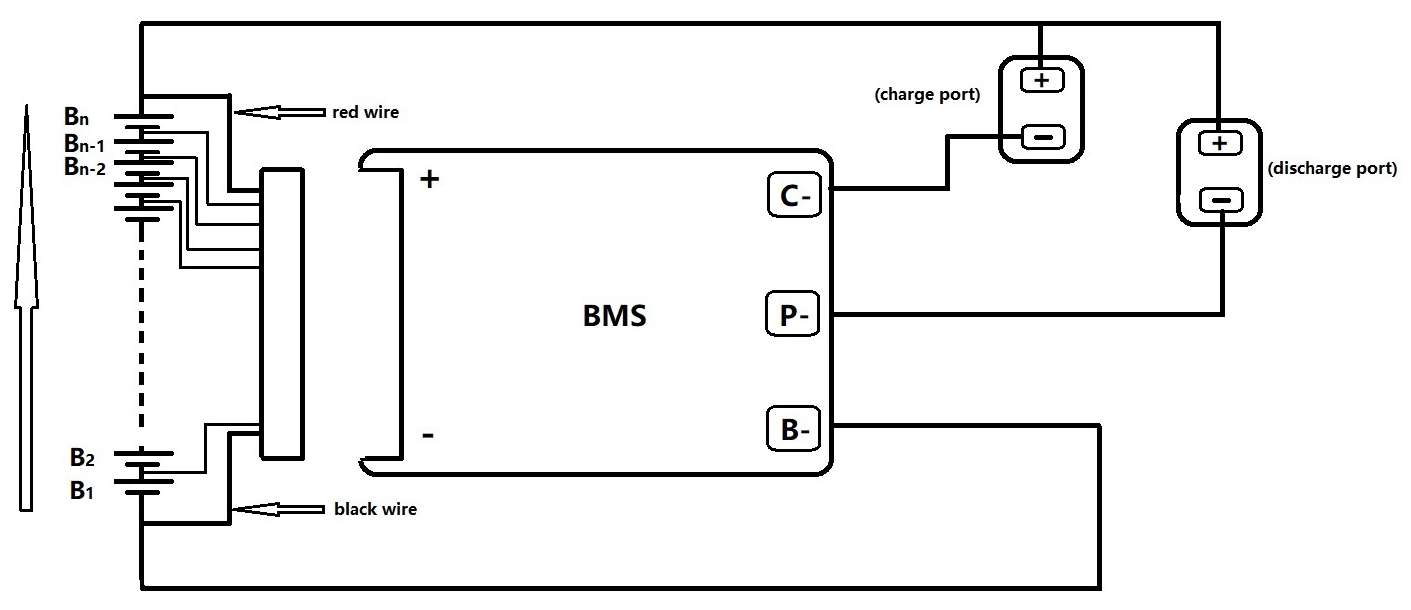
\includegraphics[width=0.75\linewidth]{figures/carga-descarga.png}
  \caption[Diagrama de un sistema de control de baterías.]{Diagrama de un sistema de control de baterías con señales de carga y descarga independientes~\cite{sunkko2025two}.}
  \label{fig:carga-descarga}
\end{figure}

¿Qué sucede entonces cuando las dos señales se activan a la vez? La activación simultanea resulta en un bloqueo mutuo donde ocurre un cortocircuito, el cual podría causar daños físicos internos a las celdas de la batería (en la practica el \gls{bms} lo impide), por esta razón la misión del sistema de control de baterías es evitar esta situación. Para ello, limita las consignas a una única señal en donde los valores positivos indican carga, los negativos descarga y cero la inactividad.

Por ejemplo, una situación en la que una carga y descarga simultanea podría suceder, de no ser por las limitaciones físicas de las baterías, se da cuando existe recurso de generación limitado por los límites de programa para un periodo beneficioso de venta, en donde la batería querría tomarlo y venderlo directamente en el mismo periodo. Visualizado en la tabla~\ref{tab:carga-descarga-simultanea}.

\begin{table}[ht]
  \centering
  \begin{tabular}{|l|S|S|S|S|}
    \hline
    Periodo & {Batería [\si{\mega\watt}]}  & {Generación [\si{\mega\watt}]}  & {Instalación [\si{\mega\watt}]}  & {Precio [\si{\text{\euro}\per\mega\watt\hour}]} \\
    \hline
    H20Q1   & 5.5                          & 32.5                            & 32.5                             & -5.00                                           \\
    H20Q2   & 5.5                          & 32.5                            & 32.5                             & 20.00                                           \\
    H20Q3   & 0.0                          &  0.0                            &  0.0                             & 53.86                                           \\
    H20Q4   & 0.0                          &  0.0                            &  0.0                             & 89.64                                           \\
    H21Q1   & 5.5                          &  0.0                            & 32.5                             & 37.24                                           \\
    H21Q2   & 5.5                          &  0.0                            & 32.5                             & 69.00                                           \\
    H21Q3   & 5.5                          &  0.0                            & 32.5                             & 85.42                                           \\
    H21Q4   & 5.5                          &  0.0                            & 32.5                             & 93.80                                           \\
    H22Q1   & 5.5                          &  0.0                            & 32.5                             & 71.00                                           \\
    H22Q2   & 5.5                          & 32.5                            & 32.5                             & 69.00                                           \\
    H22Q3   & 5.5                          & 32.5                            & 32.5                             & 69.00                                           \\
    H22Q4   & 5.5                          & 32.5                            & 32.5                             & 73.00                                           \\
    \hline
  \end{tabular}
  \caption[Límites de programa y conflictos en la exportación.]{Límite de programa donde, desde el periodo H21Q1 al H22Q1, la exportación de la generación está limitada mientras que la batería es capaz de exportar libremente, pudiendo causar conflictos entre la carga de aprovechamiento de la generación y la descarga de la venta en precios altos.}
  \label{tab:carga-descarga-simultanea}
\end{table}

Para adecuarse a dichas limitaciones físicas, se combinan las señales de carga con signo positivo y descarga con signo negativo obtenidas de la optimización y posteriormente convertidas en potencia \( P = P_{d} - P_{c} \). También se añade otra capa de prevención de desactivando previamente los periodos con carga y descarga simultanea, lo cual ciertamente puede causar desvíos en el programa, pero estos serias fácilmente solucionados en optimizaciones posteriores y nunca deberían ocurrir\footnote{Los indicadores de carga y descarga simultanea introducidos en la sección~\ref{makereference5.1.2} ya lo tienen en cuenta, pero se realiza un esfuerzo para separar las responsabilidades de los diferentes roles.}, de todos modos.

Con las posiciones transformadas en potencia, solo se toman en cuenta los cambios en el perfil de potencia y se anota el tiempo de inicio de cada cambio.

Por último, el envio de las consignas se realiza a través de la señal o punto ofrecido por el \gls{bms} configurado en el \gls{pis}, llamado \texttt{Programa} y explicado en el apartado de infraestructura~\ref{makereference3.2}. Se hace uso del mismo flujo descrito en la sección~\ref{makereference3.5} pero, en vez de leer señales, se escriben en los tiempos correspondientes en el historiador.

Cuando llegue el momento de cambio en el perfil de potencia de la batería y la señal del programa esté escrita en el historiado, este automáticamente enviará de vuelta un mensaje IEC 60870-5-104 a la estación marcando el nuevo perfil de potencia y la batería responderá correspondientemente.

Con esto, uno de los aspectos más cruciales no resulta ser precisamente la consignación de un nuevo perfil de potencia de carga o descarga, sino la vuelta al mínimo técnico. Es decir, es una absoluta necesidad hacer que la batería vuelva a un perfil de potencia nulo cuando se haya terminado la carga o descarga, de tal forma que no continúe ciclándose.

Resulta interesante destacar que, durante el despliegue del sistema en una de las instalaciones, no se llegó a consignar correctamente la vuelta al mínimo técnico de la batería debido a un fallo lógico, por lo que esta continuó cargándose más allá del límite máximo del \( \mathrm{SoC}_{\text{max}} \) establecido y, al llegar al límite de almacenamiento, hizo saltar la alarma del \gls{bms}. El problema desplomó la disponibilidad de la batería y llegó a causar pérdidas monetarias hasta rápidamente conseguir arreglarlo.

Dicha situación subraya la importancia de disponer de herramientas de observación y control manual del sistema, como la descrita en la próxima sección~\ref{makereference6.2}.

\subsection{Emisión de ofertas}
\label{makereference6.1.2}

Para emitir la oferta al mercado, es necesario calcular el precio al que ofertar la posición de la batería\footnote{La oferta del activo de generación se configura de forma manual un valor fijo \( \lambda^{O}_{\text{RES}, t} = \lambda^{O}_{\text{RES}} \), generalmente siendo \SI{0}{\text{\euro}\per\mega\watt\hour} para asegurar su casación, ya que su energía no puede ser almacenada más que en la batería misma.}. Para ello se emplea un algoritmo de desarrollo propio que permite agrupar las ofertas por ciclos.

En un primer momento, precisamente a los inicios de desarrollo de la emisión de la oferta, el precio de oferta se correspondía directamente al precio de mercado, como en la ecuación~\ref{eq:emisión-directa}.

\begin{samepage}

  \begin{equation}
    \label{eq:emisión-directa}
    \lambda^{O}_{\text{BESS}, t} = \lambda^{M}_{t}
  \end{equation}

  donde

  \begin{itemize}

    \item \( \lambda^{O}_{\text{BESS}, t} \) es el precio de oferta de la batería en el periodo \( t \) en \si{\text{\euro}\per\mega\watt\hour}.

    \item \( \lambda^{M}_{t} \) es el precio del mercado eléctrico en el periodo \( t \) en \si{\text{\euro}\per\mega\watt\hour}.

  \end{itemize}

\end{samepage}

Dicho comportamiento dispone de un fallo inaceptable en el funcionamiento del ciclado de la batería. Como el mercado eléctrico es marginalista, si existe un desvío del precio de casación a la dirección opuesta de la oferta en comparación a la predicción de precio empleada durante la operación, la oferta nunca tendrá la capacidad de casar en el mercado, resultando en un desvío de programa que, muy probablemente no podrá ser recuperado por la misma razón en los mercados posteriores.

Una solución sencilla al comportamiento previamente descrito, empleado como evolución de la lógica de emisión de ofertas del sistema, es incluir una tolerancia de oferta en el calculo del precio. La tolerancia aumenta o disminuye el precio de oferta en la dirección opuesta al beneficio en la compra o venta, buscando la casación en el mercado, ecuación~\ref{eq:emisión-tolerancia}. Este comportamiento funciona ya que permite cubrirse ante pequeños desvíos de precio y sigue sin afectar a la disminución del beneficio si el desvío de precio es favorable. En cambio, esta solución introduce un problema doble.

\begin{samepage}

  \begin{equation}
    \label{eq:emisión-tolerancia}
    \lambda^{O}_{\text{BESS}, t} =
    \begin{cases}
      \lambda^{M}_{t} + \Delta \lambda & \text{si } P_{t} < 0 \quad (\text{carga})       \\
      \lambda^{M}_{t} - \Delta \lambda & \text{si } P_{t} > 0 \quad (\text{descarga})    \\
      0                                & \text{si } P_{t} = 0 \quad (\text{estado estacionario}) \\
    \end{cases}
  \end{equation}

  donde

  \begin{itemize}

    \item \( \lambda^{O}_{\text{BESS}, t} \) es el precio de oferta de la batería en el periodo \( t \) en \si{\text{\euro}\per\mega\watt\hour}.

    \item \( \lambda^{M}_{t} \) es el precio del mercado eléctrico en el periodo \( t \) en \si{\text{\euro}\per\mega\watt\hour}.

    \item \( P_{t} \) es la potencia a mantener durante el periodo \( t \) en \si{\mega\watt}.

    \item \( \Delta \lambda \) es la tolerancia de oferta en \si{\text{\euro}\per\mega\watt\hour}.

  \end{itemize}

\end{samepage}

Primero, el uso de una tolerancia absoluta implica que el sistema solo puede defenderse ante desvíos de precio según su magnitud, pero, cuanto mayor es el precio de mercado, mayores suelen ser los desvíos de precio\footnote{Si la predicción del precio de mercado supera los \SI{100}{\text{\euro}\per\mega\watt\hour}, es más probable que el precio de casación termine en un rango de \SI{80}{\text{\euro}\per\mega\watt\hour} a \SI{120}{\text{\euro}\per\mega\watt\hour} aproximadamente, con un desvío de precio de \SI{20}{\text{\euro}\per\mega\watt\hour}. Si la predicción es de \SI{0}{\text{\euro}\per\mega\watt\hour}, lo normal es que fluctúe en un rango de \SI{-5}{\text{\euro}\per\mega\watt\hour} a \SI{5}{\text{\euro}\per\mega\watt\hour} o menos, un desvío de precio de \SI{5}{\text{\euro}\per\mega\watt\hour}, mucho menor.}. Es complicado, por no decir imposible y poco intuitivo, seleccionar dinámicamente entre una tolerancia absoluta o relativa.

Segundo, si una de las ofertas no casa, ocurre la llamada casación parcial~\cite{cnmc2024mercados}, en donde la batería mantiene un ciclo incompleto. Si el mercado acepta solo algunos de los periodos el estado de carga resultante puede no permitir completar el ciclo previsto o cumplir con compromisos posteriores.

Para evitar estos problemas, el sistema finalmente propone y hace uso del algoritmo de emisión de oferta por semiciclo de carga.

El objetivo final es agrupar los semiciclos de carga y descarga y obtener sus precios límites de compra y venta, inicialmente se calcula la diferencia entre el estado de carga de un periodo y el anterior en la ecuación~\ref{eq:diferencia-soc}.

\begin{samepage}

  \begin{equation}
    \label{eq:diferencia-soc}
    \Delta \mathrm{SoC}_{t} =
    \begin{cases}
      \mathrm{SoC}_{t} - \mathrm{SoC}_{t-1} & \text{si } t > 0 \quad (\text{horizonte de optimización}) \\
      \mathrm{SoC}_{0}                      & \text{si } t = 0 \quad (\text{periodo inicial})           \\
    \end{cases}
  \end{equation}

  donde

  \begin{itemize}

    \item \( \mathrm{SoC}_{t} \) es el \gls{soc} de la batería en el periodo \( t \) en \si{{\mega\watt\hour}}.

    \item \( \Delta \mathrm{SoC}_{t} \) es la diferencia del \gls{soc} de la batería entre periodos contiguos en \si{{\mega\watt\hour}}.

  \end{itemize}

\end{samepage}

Con ello, es posible calcular la dirección de cambio del \gls{soc} de la batería. Es decir, determinar si la batería se esta cargando, descargando o en estado estacionario, ecuación~\ref{eq:sigma-carga}. Cabe destacar que el uso del \gls{soc} es necesario, a diferencia del resto de resultados de la optimización (como la posición), ya que este representa el \textit{source of truth} del sistema.

\begin{samepage}

  \begin{equation}
    \label{eq:sigma-carga}
    \sigma_{t} =
    \begin{cases}
      +1 & \text{si } \Delta\mathrm{SoC}_{t} > 0 \quad (\text{carga})               \\
      -1 & \text{si } \Delta\mathrm{SoC}_{t} < 0 \quad (\text{descarga})            \\
      0  & \text{si } \Delta\mathrm{SoC}_{t} = 0 \quad (\text{estado estacionario}) \\
    \end{cases}
  \end{equation}

  donde

  \begin{itemize}

    \item \( \Delta \mathrm{SoC}_{t} \) es la diferencia del \gls{soc} de la batería entre periodos contiguos en \si{{\mega\watt\hour}}.

    \item \( \sigma_{t} \) es el indicador de la dirección de ciclado de la batería.

  \end{itemize}

\end{samepage}

A continuación, se calculan los llamados puntos álgidos en la ecuación~\ref{eq:puntos-algidos-inf-sup}, tanto para el \gls{soc} límite superior o inferior. Los puntos álgidos representan los baremos de consideración de los semiciclos. La razón de su existencia es simple, y es que es relativamente común encontrarse con situaciones en las que la batería realiza un semiciclo sin llegar marcar un valor exactamente correspondiente con el \gls{soc} límite.

Es extremadamente importante que el sistema se defienda ante situaciones de ciclado apenas completo, ya que puede que existan parámetros que no se correspondan estrictamente al comportamiento físico de la instalación, debido a diferencias en los decimales\footnote{En la sección~\ref{makereference5.5} se detalla el ajuste de la resolución numérica, lo que comúnmente genera ciclados incompletos, aunque la diferencia sea mínima.}. Además, permite aumentar el control de la consideración de los ciclos desde el punto de vista de los operarios de telecontrol.

\begin{samepage}

  \begin{subequations}
    \label{eq:puntos-algidos-inf-sup}

    \begin{equation}
      B_{\text{inf}, t} = \mathrm{SoC}_{t} \le \left( \frac{\mathrm{SoC}_{\text{min}}}{100} + \frac{\mathrm{SoC}_{\text{tol}}}{100} \right) \cdot E_{\text{cap}}
    \end{equation}

    \begin{equation}
      B_{\text{sup}, t} = \mathrm{SoC}_{t} \ge \left( \min\left(\frac{\mathrm{SoC}_{\text{max}}}{100}, \frac{D}{100}\right) - \frac{\mathrm{SoC}_{\text{tol}}}{100} \right) \cdot E_{\text{cap}}
    \end{equation}

  \end{subequations}

  donde

  \begin{itemize}

    \item \( \mathrm{SoC}_{t} \) es el \gls{soc} de la batería en el periodo \( t \) en \si{{\mega\watt\hour}}.

    \item \( \mathrm{SoC}_{\text{min}} \) y \( \mathrm{SoC}_{\text{max}} \) son los límites mínimo y máximo del \gls{soc} de la batería en porcentaje (\%).

    \item \( E_{\text{cap}} \) es la capacidad de almacenamiento de la batería en \si{{\mega\watt\hour}}.

    \item \( D \) es la disponibilidad de la batería en porcentaje (\%).

    \item \( \mathrm{SoC}_{\text{tol}} \) es la tolerancia del punto álgido en porcentaje (\%).

    \item \( B_{\text{inf}, t} \) y \( B_{\text{sup}, t} \) son los indicadores de los punto álgidos inferior y superiores en el periodo \( t \).

  \end{itemize}

\end{samepage}

Como no se desea contar múltiples ciclos cuando sucedan múltiples periodos contiguos que sobrepasen un punto álgido, solo se tienen en cuenta las entradas para cada la carga y descarga. Todo ello se encuentra representado en la ecuación~\ref{eq:puntos-algidos-desplazados}.

\begin{samepage}

  \begin{subequations}
    \label{eq:puntos-algidos-desplazados}

    \begin{equation}
      B_{\text{inf}, t} =
      \begin{cases}
        0                                                & \text{si } t = 0 \\
        B_{\text{inf}, t} \land \neg B_{\text{inf}, t+1} & \text{si } t > 0 \\
      \end{cases}
    \end{equation}

    \begin{equation}
      B_{\text{sup}, t} =
      \begin{cases}
        0                                                & \text{si } t = 0 \\
        B_{\text{sup}, t} \land \neg B_{\text{sup}, t+1} & \text{si } t > 0 \\
      \end{cases}
    \end{equation}

  \end{subequations}

  donde

  \begin{itemize}

    \item \( B_{\text{inf}, t} \) y \( B_{\text{sup}, t} \) son los indicadores de los punto álgidos inferior y superiores en el periodo \( t \).

  \end{itemize}

\end{samepage}

A continuación, se toman juntan los puntos álgidos inferiores y superiores en la ecuación~\ref{eq:puntos-algidos}. La razón de realizar las operaciones por separado es impedir situaciones de cargas o descargas muy rápidas, donde se sobrepasen puntos álgidos distintos (a diferencia de la ecuación~\ref{eq:puntos-algidos-desplazados}) en periodos contiguos. Dentro del funcionamiento normal de las baterías, no es precisamente una situación que ocurra muy a menudo, pero es técnicamente posible que suceda, sobre todo en mercados de menor granularidad.

\begin{samepage}

  \begin{equation}
    \label{eq:puntos-algidos}
    B_{t} = B_{\text{inf}, t} \lor B_{\text{sup}, t}
  \end{equation}

  donde

  \begin{itemize}

    \item \( B_{\text{inf}, t} \) y \( B_{\text{sup}, t} \) son los indicadores de los punto álgidos inferior y superiores en el periodo \( t \).

    \item \( B_{t} \) es el indicador de punto álgido en el periodo \( t \).

  \end{itemize}

\end{samepage}

Junto a ello, se desplazan los puntos un periodo en el tiempo para resolver problemas causados por \textit{off-by-one errors}. Se representa en la ecuación~\ref{eq:puntos-algidos-shift}.

\begin{samepage}

  \begin{equation}
    \label{eq:puntos-algidos-shift}
    B_t =
    \begin{cases}
      0       & \text{si } t = 0 \\
      B_{t+1} & \text{si } t > 0 \\
    \end{cases}
  \end{equation}

  donde

  \begin{itemize}

    \item \( B_{t} \) es el indicador de punto álgido en el periodo \( t \).

  \end{itemize}

\end{samepage}

Con los puntos álgidos correctamente identificados, se toma una cuenta acumulativa de los mismos. Cada número de la cuenta proporciona indirectamente un identificador unívoco sucesivo del semiciclo realizado (semiciclo 1, semiciclo 2, \ldots), en la ecuación~\ref{eq:conteo-ciclos}.

\begin{samepage}

  \begin{equation}
    \label{eq:conteo-ciclos}
    N_{t} = 1 + \sum_{i=0}^{t-1} B_{i}
  \end{equation}

  donde

  \begin{itemize}

    \item \( B_{i} \) es el indicador de punto álgido en el periodo \( i \).

    \item \( N_{t} \) es el contador acumulado de semiciclos en el periodo \( t \).

  \end{itemize}

\end{samepage}

Tan solo dista multiplicar el conteo de los semiciclos, correspondiente con sus identificadores, con la dirección en la que operan en la ecuación~\ref{eq:conteo-ciclos-signo}. De esta forma, a cada semiciclo se le corresponde un identificador y el signo del identificador indica el tipo de ciclo, carga, descarga o estado estacionario (positivo, negativo y cero, respectivamente).

\begin{samepage}

  \begin{equation}
    \label{eq:conteo-ciclos-signo}
    C_{t} = \sigma_{t} \cdot N_{t}
  \end{equation}

  donde

  \begin{itemize}

    \item \( \sigma_{t} \) es el indicador de la dirección de ciclado de la batería.

    \item \( N_{t} \) es el contador acumulado de semiciclos en el periodo \( t \).

    \item \( C_{t} \) es el identificador del semiciclo con signo en el periodo \( t \).

  \end{itemize}

\end{samepage}

Finalmente, se agrupan los precios de mercado por los periodos correspondientes a cada semiciclo, ecuación~\ref{eq:agrupado-periodos}.

\begin{samepage}

  \begin{equation}
    \label{eq:agrupado-periodos}
    G_{c} = \{ \lambda^{M}_{t} \mid C_{t} = c \}
  \end{equation}

  donde

  \begin{itemize}

    \item \( C_{t} \) es el identificador del semiciclo con signo en el periodo \( t \).

    \item \( c \) es un identificador específico de semiciclo.

    \item \( \lambda^{M}_{t} \) es el precio del mercado eléctrico en el periodo \( t \) en \si{\text{\euro}\per\mega\watt\hour}.

    \item \( G_{c} \) es el conjunto de todos los precios de mercado \( \lambda^{M}_{t} \) que pertenecen a un mismo semiciclo con identificador \( c \).

  \end{itemize}

\end{samepage}

Con ello, por cada grupo, se toma el precio más bajo entre los periodos de descarga y el más alto entre los de carga, añadiendo una tolerancia absoluta en la dirección opuesta al beneficio de la oferta. Esto significa que todos los periodos de un mismo semiciclo de descarga tendrán el precio menor de venta del mercado durante dicho semiciclo, mientra que exactamente lo opuesto para la carga.

\begin{samepage}

  \begin{equation}
    \lambda^{O}_{\text{BESS}, t} =
    \begin{cases}
      \max(G_{c}) + \Delta \lambda & \text{si } c > 0 \quad (\text{carga})\\
      \min(G_{c}) - \Delta \lambda & \text{si } c < 0 \quad (\text{descarga})\\
      0                            & \text{si } c = 0 \quad (\text{estado estacionario})
    \end{cases}
  \end{equation}

  donde

  \begin{itemize}

    \item \( G_{c} \) es el conjunto de todos los precios de mercado \( \lambda^{M}_{t} \) que pertenecen a un mismo semiciclo con identificador \( c \).

    \item \( \lambda^{O}_{\text{BESS}, t} \) es el precio de oferta de referencia calculado para el semiciclo \( c \) en \si{\text{\euro}\per\mega\watt\hour}.

    \item \( \Delta \lambda \) es la tolerancia de precio para las ofertas en \si{\text{\euro}\per\mega\watt\hour}.

  \end{itemize}

\end{samepage}

La emisión de oferta por semiciclo de carga evita aceptaciones parciales y refleja las restricciones intertemporales y costes de oportunidad de la batería en forma de todo o nada. Es decir, se hace uso del comportamiento más agresivo en busca de la casación en todo momento, los bloques de ofertas por semiciclo casan en todos a la vez o ninguno, siendo esta la clave.

Es inevitable generar desvíos si el bloque no casa pero, inteligentemente, estos desvíos no se ven afectados por los subsecuentes movimientos en los mercados posteriores. Intentar solucionar el desvío no puede aumentarlo si se hace uso de esta estrategia, a diferencia de las anteriores.

Finalmente, la oferta se comunica con la herramienta externa de resolución de ofertas de la entidad energética en el formato adecuado\footnote{La emisión de ofertas del sistema soporta múltiples formatos, pero solo se muestra el usado en producción.}, véase la tabla~\ref{tab:formato-oferta}. Si no es modificada, entrará automáticamente a mercado.

\begin{table}[ht]
  \centering
  \resizebox{\textwidth}{!}{
    \begin{tabular}{|c|c|c|c|l|S|S|S|}
      \hline
      FECHA      & PERIODO & COD\_RESOLUCION & BLOQUE & UFI   & {ENERGIA} & {POTENCIA} & {PRECIO} \\
      \hline
      05/09/2025 & 29      & 15M             & 1      & ABADC & -1.3      & -5.2       &  4.92    \\
      05/09/2025 & 30      & 15M             & 1      & ABADC & -1.3      & -5.2       &  4.92    \\
      05/09/2025 & 31      & 15M             & 1      & ABADC & -1.3      & -5.2       &  4.92    \\
      05/09/2025 & 32      & 15M             & 1      & ABADC & -1.1      & -4.4       &  4.92    \\
      05/09/2025 & 85      & 15M             & 1      & ABADV &  1.3      &  5.2       & 80.40    \\
      05/09/2025 & 86      & 15M             & 1      & ABADV &  1.3      &  5.2       & 80.40    \\
      05/09/2025 & 87      & 15M             & 1      & ABADV &  1.3      &  5.2       & 80.40    \\
      05/09/2025 & 88      & 15M             & 1      & ABADV &  1.1      &  4.4       & 80.40    \\
      \hline
    \end{tabular}
  }
  \caption[Formato de oferta de mercado.]{Formato de oferta de mercado.}
  \label{tab:formato-oferta}
\end{table}

\section{Cuadro de mando}
\label{makereference6.2}

Aunque el sistema desarrollado sea completamente agnóstico de ningún tipo de intervención manual para su operación, en algunas ocasiones no es capaz de tener en cuenta todos los factores que afectan a la totalidad de los componentes involucrados, conocidos por los agentes de mercado.

Además, una de las situaciones problemáticas más comunes, encontradas a la hora de realizar el despliegue, se corresponde con las indisponibilidades manuales o programadas de la batería. Estas indiponibilidades no son causadas precisamente por las señales integradas de disponibilidad de los \glspl{bess}, descritas anteriormente en la sección~\ref{makereference3.2}, sino por pruebas de integración del sistema. Por ello, los operadores de telecontrol necesitan cerciorarse de algún modo que la batería siga las consignas dadas.

Principalmente motivado por dicho propósito y con el objetivo de facilitar la observabilidad de la infraestructura, se desarrolla un cuadro de mando, como se ve en la figura~\ref{fig:cuadro-de-mando}, para la unificación completa del control de la operación del sistema, desde la simulación de las operaciones, la consignación manual y asistida, la modificación de los parámetros operativos y la priorización de programas.

\begin{figure}
  \centering
  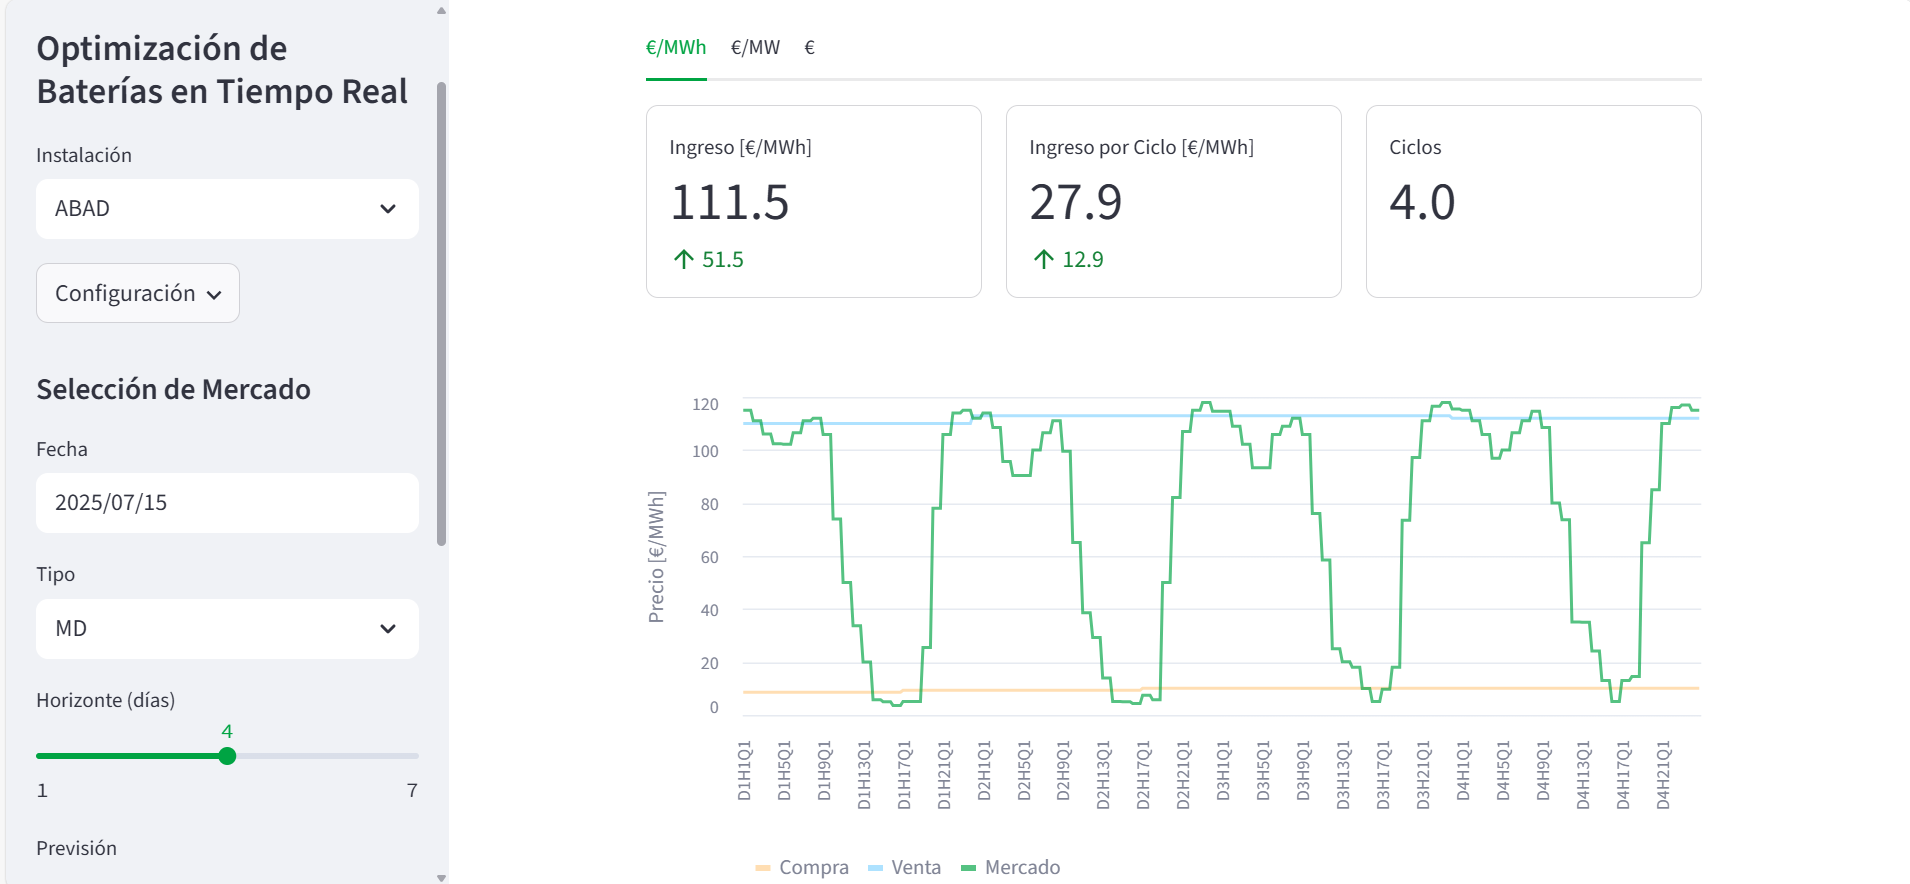
\includegraphics[width=0.75\linewidth]{figures/cuadro-de-mando.png}
  \caption[Cuadro de mando del sistema.]{Cuadro de mando del sistema.}
  \label{fig:cuadro-de-mando}
\end{figure}

De esta forma, el cuadro de mando del sistema es la pieza cable mediante la cual los agentes de mercado y operadores de telecontrol son capaces de interactuar con las baterías, en tiempo real, con el objeto de modificar su comportamiento como les convenga. A los agentes de mercado se les da la posibilidad de cambiar las posiciones en busca de una mejor oportunidad de arbitraje, impulsada por factores externos que escapen al control del sistema, y los operadores de telecontrol pueden realizar pruebas de ciclado de las baterías, sin tener que interactuar con el \gls{rtu} y los protocolos de comunicación correspondientes. En ello reside el valor principal del desarrollo del cuadro de mandos.

Cabe destacar que, más allá del cuadro de mando del comando y control orientado a los agentes de mercado y operadores de telecontrol, cada componente del sistema también es capaz de ser configurado mediante canales no interactivos si es necesario, estando estos orientadas a los operadores de telecontrol para la configuración de la infraestructura operativa, al personal de sistemas para el entorno de mercado, y a los agentes de mercado para la modelización estructural.

\subsection{Funcionalidad principal}
\label{makereference6.2.1}

El cuadro de mando ha sido desarrollado en la misma tecnología principal utilizada en la mayoria de los otros componentes, Python. Esta vez, se hace uso de Streamlit~\cite{streamlit2025faster}, un componente para construir herramientas interactivas.

Tras pasar por un servicio de autenticación que únicamente permite el acceso a agentes de mercado y operadores de telecontrol designados, el usuario es presentado con la interfaz de operación principal.

En ella, es posible modificar la configuración operativa de cada una de las instalaciones, establecer la situación de mercado concreta a tener en cuenta y cambiar la fuente de los precios marginales explicados en la sección~\ref{makereference4.1.1}, entre otras acciones mostradas en la figura~\ref{fig:configuracion-sistema}.

\begin{figure}
  \centering
  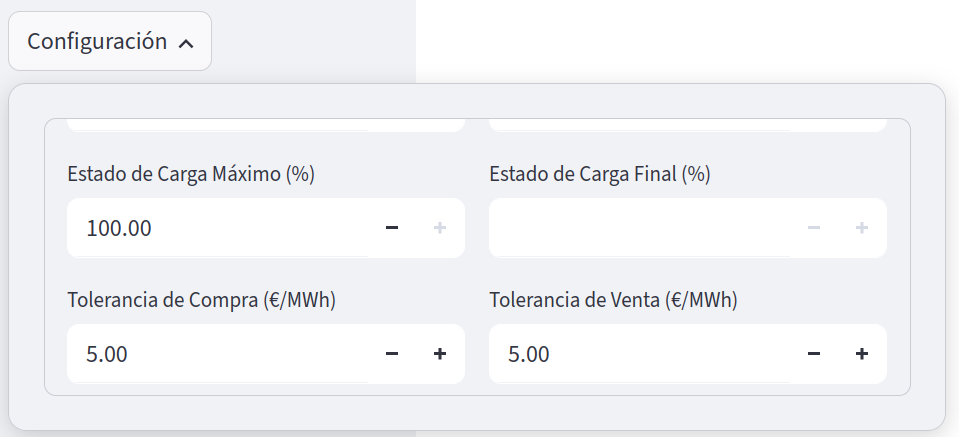
\includegraphics[width=0.5\linewidth]{figures/configuracion-sistema.png}
  \caption[Configuración del sistema.]{Configuración del sistema interactiva a través del cuadro de mandos.}
  \label{fig:configuracion-sistema}
\end{figure}

Todo esto permite realizar simulaciones tanto a pasado y a futuro del comportamiento del sistema y de la evolución del mismo a lo largo del ciclo de vida de los mercados. Es decir, un agente de mercado es capaz de comprender fácilmente no solo lo que va a suceder el día de mañana en el mercado diario, sino también en los subsecuentes mercado intradiarios e incluso en las sesiones del mercado intradiario continuo, y ver la evolución de las posiciones.

Junto a ello, se permite importar datos del mercado localmente y obviar todo el capítulo~\ref{makereference3} del entorno de mercado, con el propósito de permitir el uso del cuadro de mandos en situaciones en donde la información no esté disponible o se quiera modificar manualmente. Precisamente, en sinergia con la característica de exportar la información del entorno de mercado una vez obtenida, es posible realizar simulaciones más avanzadas donde todos los aspectos de entrada al sistema (incluso las señales de la infraestructura a través de la configuración de las instalaciones) sean capaces de ser modificadas.

Además, el entorno de mercado no es la única información capaz de ser exportada. Los resultados del programa óptimo de la batería, obtenido tras realizar todo el proceso, pueden ser descargados en un formato CSV con el fin de inspeccionarlos detalladamente, o incluso modificarlos (aunque resulte más intuitivo realizar cualquier modificación a través del cuadro de mandos directamente).

También se permite especificar tanto un programa, en donde se realize el seguimiento del programa mismo y la solución del modelado estructural del capítulo~\ref{makereference4} se desactive, como un objetivo de \gls{soc}, en donde el sistema cumpla con las indicaciones en los periodos determinados pero siga realizando la tarea de optimización, representado en la figura~\ref{fig:soc-manual}. Resulta crucial que todo el resto de validaciones siguan en funcionamiento, por lo que no es posible introducir un programa invalido de ningún modo. Con esto, se observa como la inclusión del objetivo de la modularización del sistema resulta más que beneficiosa ante dichas situaciones.

\begin{figure}
  \centering
  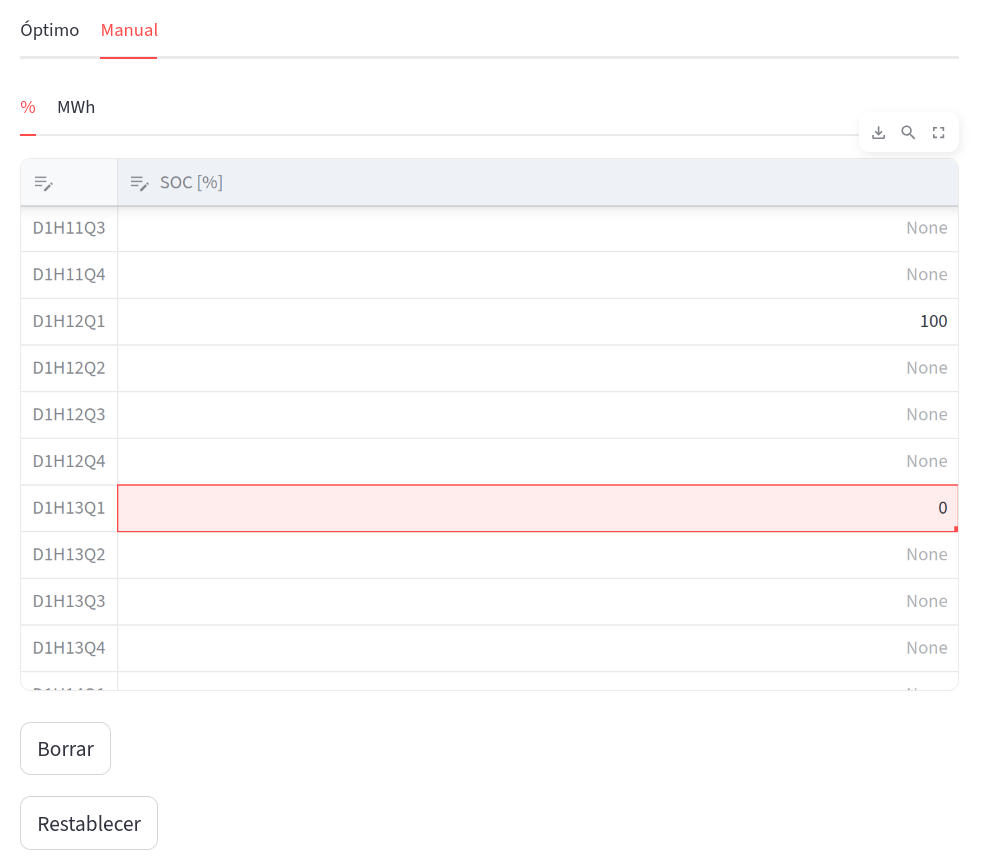
\includegraphics[width=0.5\linewidth]{figures/soc-manual.png}
  \caption[Regulación manual del estado de carga.]{Regulación manual del estado de carga, en donde se ejemplifica la introducción de un posible periodo de prueba, en el que un operador de telecontrol busque ciclar la batería completamente a medio día.}
  \label{fig:soc-manual}
\end{figure}

En colación, es posible activar o desactivar el modo de funcionamiento automático y sustituirlo por un modo de funcionamiento manual, característica más que relevante para asegurar el cumplimiento de un programa concreto ante fallos o pruebas. Desactivado, el sistema hace caso de los programas manuales obtenidos mediante el cuadro de mandos, activado en cambio, lo sobrescribe.

Finalmente, se presentan los \gls{kpi} en forma de los ingresos obtenidos por energía vendida, los ingresos totales y los ciclos realizado en diferentes unidades, dirigidos a los agentes de mercado, figura~\ref{fig:kpi-sistema}. También se muestra el perfil de generación para las instalaciones híbridas, figura~\ref{fig:perfil-generacion}, junto al programa óptimo de la batería, figura~\ref{fig:programa-optimo}, su \gls{soc} a lo largo del horizonte de optimización, figura~\ref{fig:soc-bess}, y las limitaciones técnicas si son aplicables, figura~\ref{fig:limitaciones-tecnicas}.

\begin{figure}
  \centering
  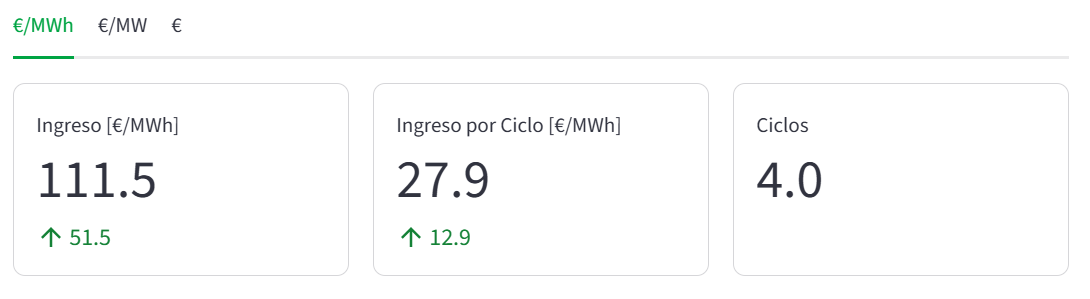
\includegraphics[width=0.75\linewidth]{figures/kpi-sistema.png}
  \caption[Indicadores de rendimiento.]{Indicadores de rendimiento.}
  \label{fig:kpi-sistema}
\end{figure}

\begin{figure}
  \centering
  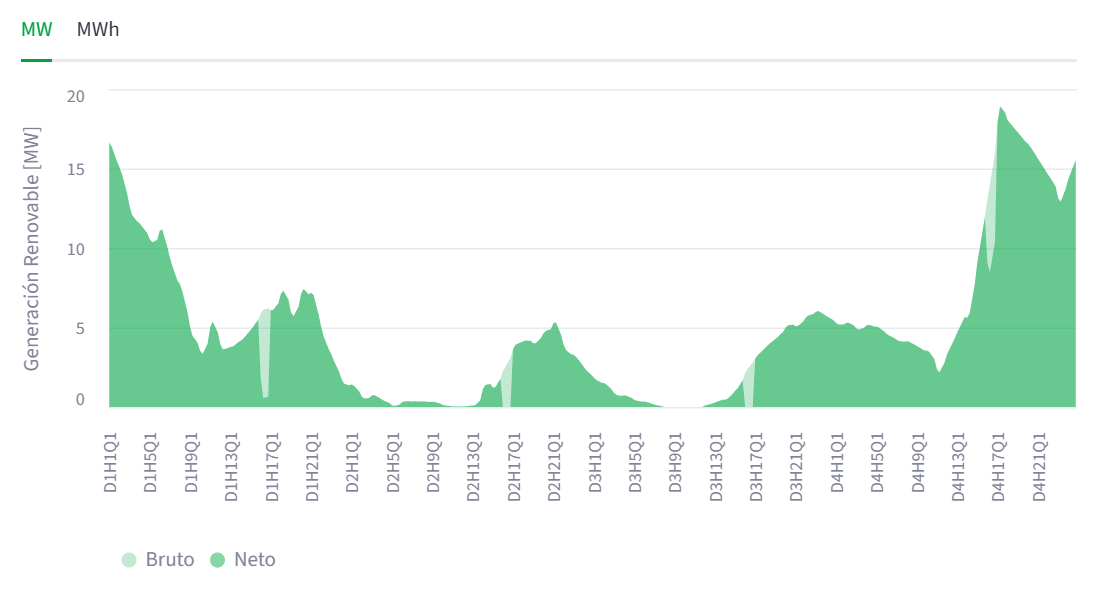
\includegraphics[width=0.75\linewidth]{figures/perfil-generacion.png}
  \caption[Perfil de generación.]{Perfil de generación.}
  \label{fig:perfil-generacion}
\end{figure}

\begin{figure}
  \centering
  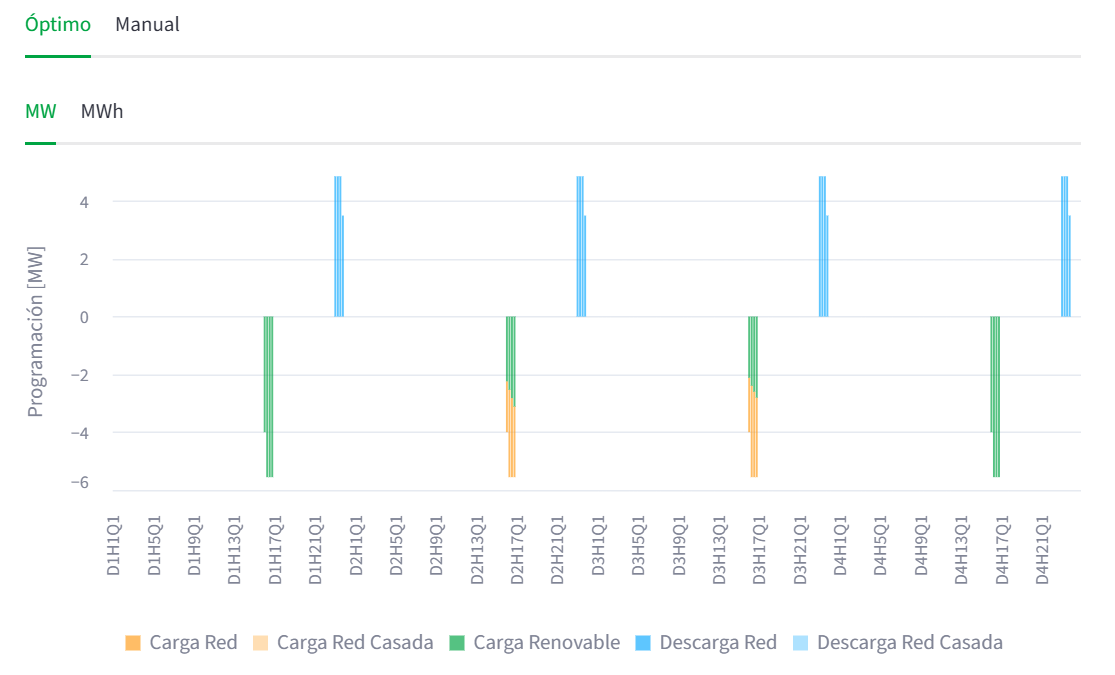
\includegraphics[width=0.75\linewidth]{figures/programa-optimo.png}
  \caption[Programa óptimo de la batería.]{Programa óptimo de la batería.}
  \label{fig:programa-optimo}
\end{figure}

\begin{figure}
  \centering
  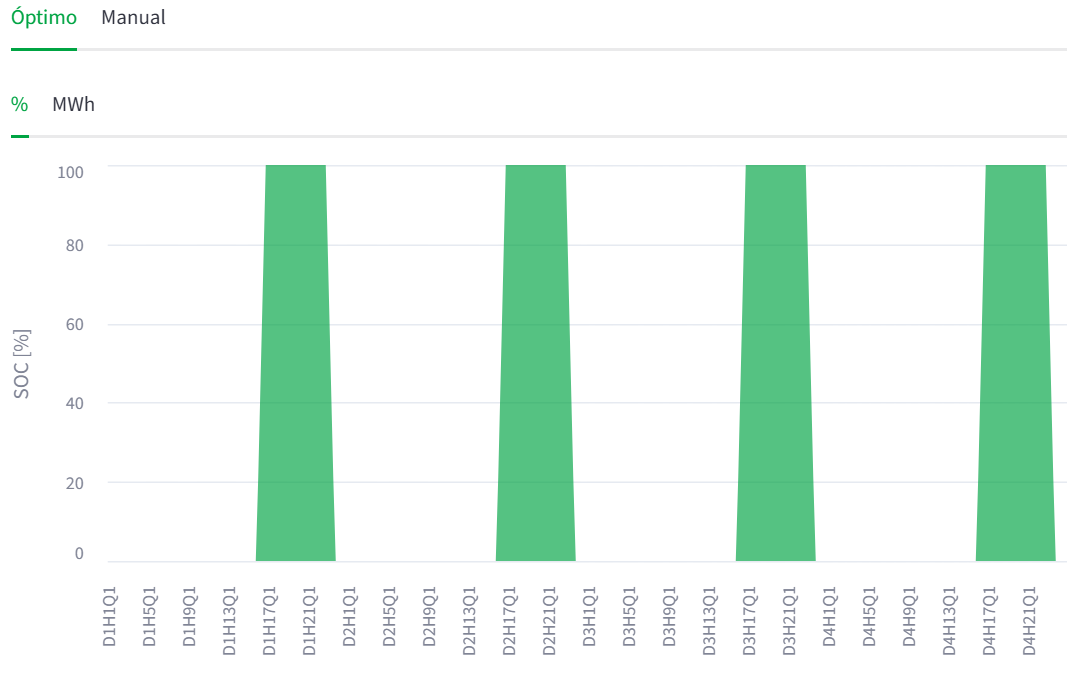
\includegraphics[width=0.75\linewidth]{figures/soc-bess.png}
  \caption[Estado de carga de la batería.]{Estado de carga de la batería.}
  \label{fig:soc-bess}
\end{figure}

\begin{figure}
  \centering
  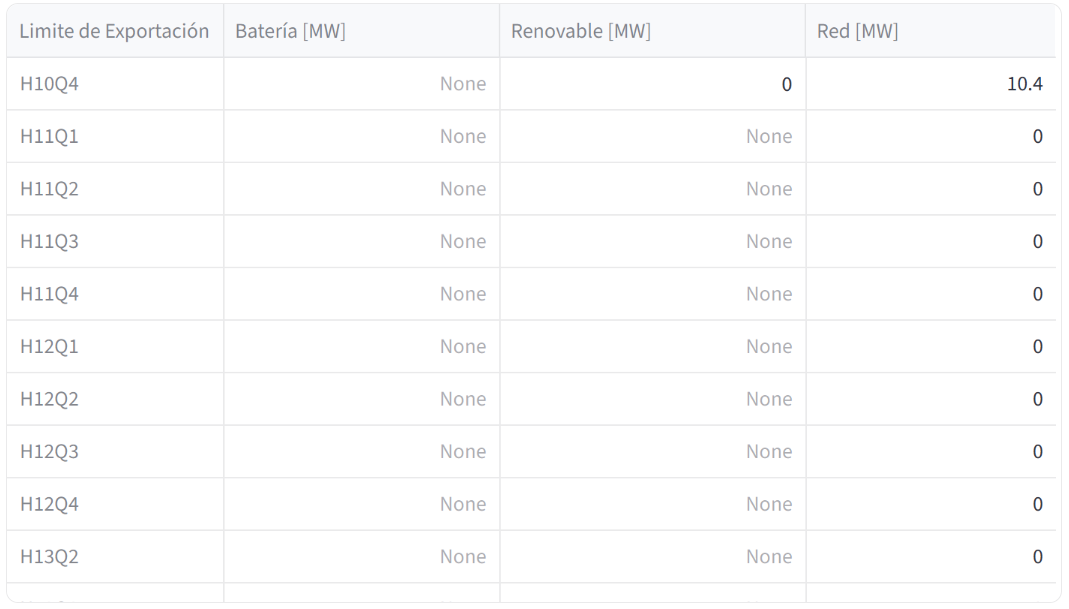
\includegraphics[width=0.75\linewidth]{figures/limitaciones-tecnicas.png}
  \caption[Limitaciones técnicas de la instalación.]{Limitaciones técnicas de la instalación.}
  \label{fig:limitaciones-tecnicas}
\end{figure}
